\subsection{The Second Marker}\label{sec:full_marker2}
The second marker, seen in figure \ref{marker:circle}, contains three blue circles and one red circle in a green square.
First the image is split into a red, green and blue channel using HSV.
When using HSV to select for colors, hue is the dominating factor.
%The hue is selected by giving an interval in degrees from the circle.
The hue is selected as shown in figure \ref{fig:hsv_color_segmentation}.
The saturation is chosen so it selects high values as saturated red, green and blue is desired.
The intensity is not important as the ideal marker gives full intensity of the colors and the real images will give a lower intensity.

\begin{figure}[h]
\centering
\def\scalingFactor{0.4}
\begin{tikzpicture}[scale=\scalingFactor, every node/.style={scale=\scalingFactor}]
 \node[name=whole] at (-0.12,-0.05) {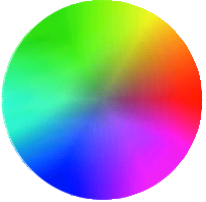
\includegraphics[scale=1]{graphics/hue} };
\end{tikzpicture}
%
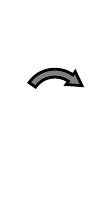
\begin{tikzpicture}[scale=\scalingFactor, every node/.style={scale=\scalingFactor}]
\node at (0,-2.2) {};
\node at (0, 2.2) {};
\def\startAngle{140}
\def\stopAngle{50}
  \draw[rotate=5,fill=gray,line width=1pt] (\startAngle:1cm) arc(\startAngle:\stopAngle:1cm) -- (\stopAngle:1.125cm) -- (0.9,0.4) -- (\stopAngle:.625cm) -- (\stopAngle:.75cm) arc (\stopAngle:\startAngle:.75cm)--cycle;
\end{tikzpicture}
%
\begin{tikzpicture}[scale=\scalingFactor, every node/.style={scale=\scalingFactor}]
 \node at (-0.12,-0.05) {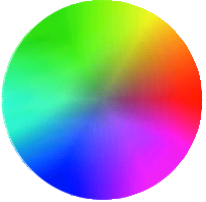
\includegraphics[scale=1]{graphics/hue} };
 \node[name=hsv, draw, thick , circle, minimum width =5.3cm] at (0,0) {};
% % % % RED % % % %
\def\MaxSat{2.8cm}
\def\MinHueR{0} 
\def\MaxHueR{30}
\def\MinSatR{1.6cm} % 0 - 1 => 0 - 2.65
 \draw (hsv.\MinHueR) -- (hsv.center) -- (hsv.\MaxHueR);
 \draw[very thick]   ([shift=(\MinHueR:\MinSatR)] hsv.center) arc(\MinHueR:\MaxHueR:\MinSatR);
% % % % GREEN % % % %
\def\MinHueG{70} 
\def\MaxHueG{145}
\def\MinSatG{1.6cm} % 0 - 1 => 0 - 2.65
 \draw (hsv.\MinHueG) -- (hsv.center) -- (hsv.\MaxHueG);
 \draw[very thick]   ([shift=(\MinHueG:\MinSatG)] hsv.center) arc(\MinHueG:\MaxHueG:\MinSatG);
% % % % BLUE % % % %
\def\MinHueB{210} 
\def\MaxHueB{270}
\def\MinSatB{1.6cm} % 0 - 1 => 0 - 2.65
 \draw (hsv.\MinHueB) -- (hsv.center) -- (hsv.\MaxHueB);
 \draw[very thick]   ([shift=(\MinHueB:\MinSatB)] hsv.center) arc(\MinHueB:\MaxHueB:\MinSatB);

 \fill[color=white]  (hsv.center) -- (0:\MinSatR) arc(0:360:\MinSatR);
 
 \fill[color=white]  (hsv.center) -- (\MaxHueR:\MaxSat) arc(\MaxHueR:\MinHueG:\MaxSat);
 \fill[color=white]  (hsv.center) -- (\MaxHueG:\MaxSat) arc(\MaxHueG:\MinHueB:\MaxSat);
 \fill[color=white]  (hsv.center) -- (\MaxHueB:\MaxSat) arc(\MaxHueB:360:\MaxSat);
\end{tikzpicture}
\caption{Hue and Saturation thresholds applied to HSV to segment colors.}
\label{fig:hsv_color_segmentation}
\end{figure}

The circles are then found by using a Hough transform for circles on the green channel.
The green channel will create a void, and thus edges, where the red and blue circles are found.
This is less expensive than finding circles on two channels and hence applied first.
The color of the circles can then be found using the center point of the circle and lookup if this point is defined as blue or red in one of the two thresholded images found earlier.
During evaluation of this method, it was found that this method sometimes missed a red or a blue circle.
This could be saved by doing an extra Hough transform on the corresponding channel and find the circle there.
This leads to potentially running the Hough transform three times so the timing of this function can wary.
%If finding the marker is more important than keeping the real time constraints.

In order to deal with projection, the Hough transform must allow more edges to be viewed as circles.
This means that more circles will be found.
In order to remove the wrong circles that are either blue or red, the surrounding points are analyzed.
If these are not found to be green, the circle is removed.

The detector was tested to find four correct points in the marker in 30/30 images in the easy set and in 50/52 images in the hard set.
The situations in which the marker was not found, was when the marker was projected so far that the center of the Hough circle was not inside the circle of the marker as seen in figure \ref{fig:circle_detection_worstcase}.

In figure \ref{fig:circle_detection} is a normal case from the easy and a worst case example from the hard set shown.
As the robot follows the point, it is not expected to be this bad at any situation so the detector is deemed successful.

\begin{figure}[h]
 \centering
 \begin{subfigure}{\exampleWidth}
 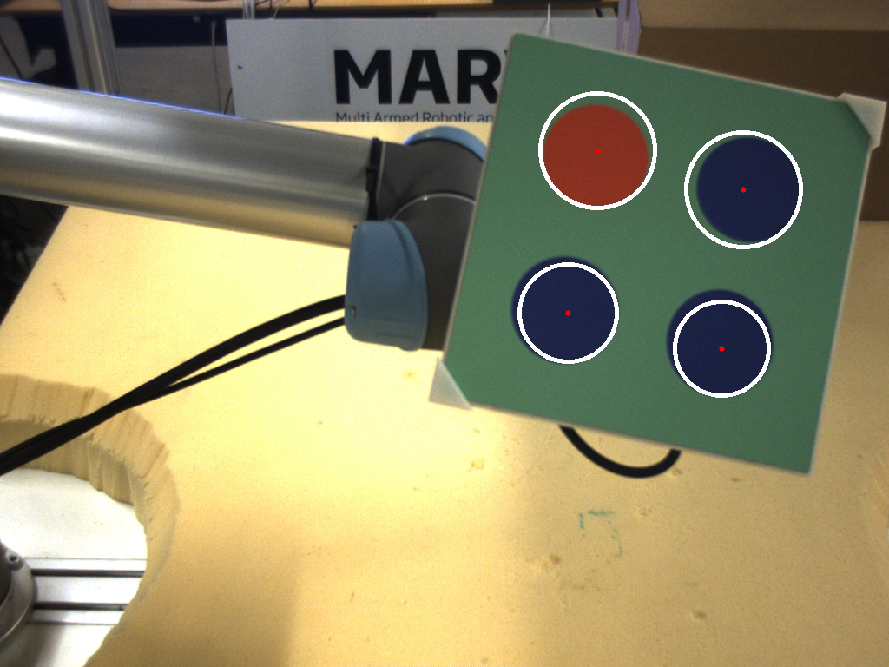
\includegraphics[width=\linewidth]{graphics/best_case_hough_circle}
 \caption{Normal case.}
 \end{subfigure}
 \begin{subfigure}{\exampleWidth}
 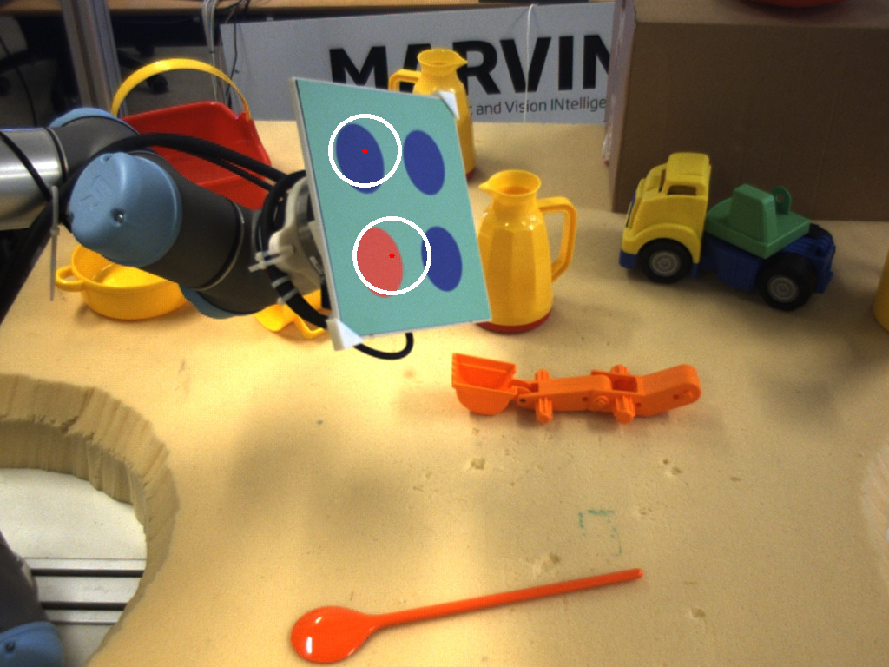
\includegraphics[width=\linewidth]{graphics/worst_case_hough_circle}
 \caption{Worst case.}
 \label{fig:circle_detection_worstcase}
 \end{subfigure}
 \caption{Detecting circles with and without projection.}
 \label{fig:circle_detection}
\end{figure}


